\begin{figure}
    \centering
    \subfloat[Number of GSS edges.]{
        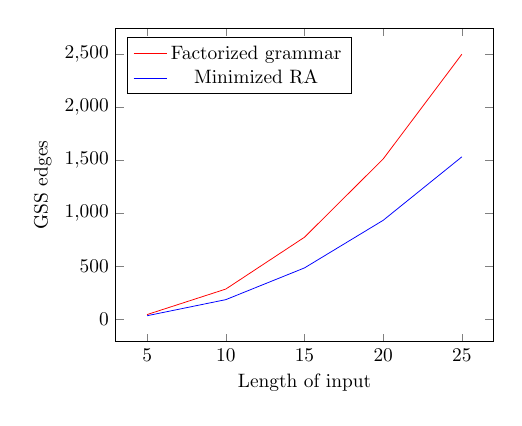
\begin{tikzpicture}[scale=0.7]
        \begin{axis}[
        legend pos = north west,
        xlabel = {Length of input},
        ylabel = {GSS edges}
        ]
        \addplot [mark=none, red] coordinates {
            (5,43) (10,284) (15,774) (20,1514) (25,2504)% (30,4477544)
        };
        \addplot [mark=none, blue] coordinates {
            (5,32) (10,184) (15,484) (20,934) (25,1534)% (30,2985034)
        };
        \legend{ 
            Factorized grammar, 
            Minimized RA
        };
        \end{axis}
        \end{tikzpicture}
        \label{fig:GSSedges}
    }
    ~
    \subfloat[Time of parsing without SPPF construction.]{
        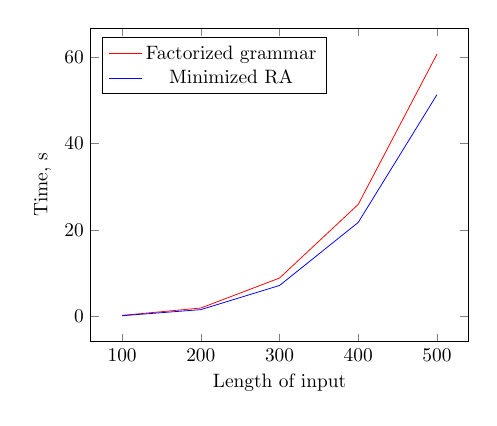
\begin{tikzpicture}[scale=0.7]
        \begin{axis}[
        legend pos = north west,
        xlabel = {Length of input},
        ylabel = {Time, s}
        ]
        \addplot [mark=none, red] coordinates {
            (100,0.206) (200,1.909) (300,8.844) (400,25.876) (500,60.617)% (1000,842.779)
        };
        \addplot [mark=none, blue] coordinates {
            (100,0.127) (200,1.54) (300,7.125) (400,21.707) (500,51.245)% (1000,768.853)
        };
        \legend{ 
            Factorized grammar, 
            Minimized RA
        };
        \end{axis}
        \end{tikzpicture}
        \label{fig:Time}
    }
    \caption{Experiments results(1).}
    \label{expPlots1}
\end{figure}